
\documentclass[runningheads,a4paper]{llncs}

\usepackage{amssymb}
\setcounter{tocdepth}{3}
\usepackage{graphicx}

\usepackage{url}
\urldef{\mailsa}\path|{matthew.patrick, manuel.oriol}@cs.york.ac.uk|
\newcommand{\keywords}[1]{\par\addvspace\baselineskip
\noindent\keywordname\enspace\ignorespaces#1}

\begin{document}

\mainmatter  % start of an individual contribution

% first the title is needed
\title{Using Random Search to Identify Fault Characteristics in Software Applications}

% a short form should be given in case it is too long for the running head
\titlerunning{Random Search and Fault Characteristics}

% the name(s) of the author(s) follow(s) next
%
% NB: Chinese authors should write their first names(s) in front of
% their surnames. This ensures that the names appear correctly in
% the running heads and the author index.
%
\author{Matthew Patrick \and Manuel Oriol}
%
\authorrunning{Random Search and Fault Characteristics}
% (feature abused for this document to repeat the title also on left hand pages)

% the affiliations are given next; don't give your e-mail address
% unless you accept that it will be published
\institute{University of York, UK\\
\mailsa\\
\url{http://www.scs.york.ac.uk}}

%
% NB: a more complex sample for affiliations and the mapping to the
% corresponding authors can be found in the file "llncs.dem"
% (search for the string "\mainmatter" where a contribution starts).
% "llncs.dem" accompanies the document class "llncs.cls".
%

\toctitle{Random Search and Fault Characteristics}
\tocauthor{Authors' Instructions}
\maketitle


\begin{abstract}
Search-based testing can be difficult for commercial applications of software because of the many potential points of failure. It is useful to have heuristics in order to guide the search. However, the majority of research on test data generation techniques focuses on small test programs that are not representative of the larger systems often used in industry. This research uses random testing to reveal run-time errors in commonly used open source software. The aim is to determine whether the fault characteristics of software differ according to its application and by doing so provide some insight into the problem of testing software applications in general.
\keywords{Random testing; Fault characteristics; YETI}
\end{abstract}


\section{Introduction}
Random search is one of the most straightforward and inexpensive testing strategies \cite{ince_1987}. It is sometimes seen as inferior to other strategies because it does not take into account  the syntactic or semantic structure of a program \cite{myers_2004}. However, because it covers the whole input-space, it is useful for providing confidence in the general characteristics of software \cite{hamlet_1994}. Its low overhead also means that random search can reveal more faults per unit of time than an exhaustive strategy \cite{mankefors_2003}. Successful automation of random testing requires an oracle that does not need human involvement to verify the results of executing each test case \cite{ince_1987}. Unfortunately, it might be just as difficult to produce an oracle that works correctly as to develop the software without any bugs.

The York Extendible Testing Infrastructure (YETI) provides a framework for executing random testing sessions without the need for an explicit oracle. The oracle is implicit in the occurrence of assertion violations and run-time errors, for example an incorrect casting or division by zero. As YETI is programming language independent, it can be used to test software written in a number of different programming languages. However, for this research it will be used to test software written in Java. YETI is able to produce a significant amount of test data in a short space of time. In Java, it is able to make up to $10^6$ calls per minute \cite{oriol_2010}. Therefore, it is very useful for providing thorough fault characteristics for the software under test. This research uses YETI to assess software used for different purposes. The results are then analysed to provide some insight into how each application area may best be tested.

\section{Categories of Software}
The aim in defining these categories of software is to work towards a benchmark from which the practices of testing each category can be improved. Software categories can be helpful if they reveal unique challenges that are faced testing examples of their software. Many of the tools developed in research are evaluated using artificial example programs that are too small-scale to be representative of any particular category. Yet in order for a tool to be relevant for industry, it must be able to perform well with much more complicated software. Therefore, we will consider how software that is used in industry may be categorised for the purposes of testing. Considerations can be made for size, the number of modules or complexity of data structures, and the way it is developed, whether the software is open source or object orientated. These categories can be useful, but they focus on the details and structure of the code rather than the purpose of the software. 

At the other end of the spectrum lie categorisations of domains in which software is intended to be used. A good example can be found in the Microsoft Asset Inventory Service \cite{microsoft_2010}. Although its categories are clearly defined by purpose, their complexity makes them difficult to distinguish from the perspective of testing. For example, the \emph{Education and Reference} and \emph{Home and Entertainment} categories both involve strong elements of user interaction that must be tested. We propose to find a compromise by considering five distinct forms of behaviour that software can exhibit: functional, open, progressive, user and timed. It is likely that some software will exhibit more than one form of behaviour. For example, a web-based application that includes a database will act progressively, but also feature open and user-type behaviour. Therefore, these categories do not represent the complete behaviour of a software system, but they do offer an insight into the types of behaviour that can be tested in software.
\newline
\textbf{Functional behaviour} involves significant numerical calculation and/or algorithmic operations. Examples range from core data structures such as \emph{java.Integer}, up to complex libraries such as the \emph{Bouncy Castle} cryptography suite. This is the kind of behaviour that is often targeted in traditional testing research.
\newline
\textbf{Open behaviour} makes use of features that are shared between multiple parties, with potentially different goals. This involves danger from attackers outside the system and the possibility of conflict between different modules inside the system. It is important that the software possesses fault tolerance and is able to resist tampering.
\newline
\textbf{Progressive behaviour} maintains and develops a data source over time. When a progressive system starts with a data source in a particular state, it must leave it in a legal state. This can be difficult, as the data source may potentially be infinite, or only bounded by the available memory. Typically, this is addressed by dividing the data source into manageable sections, for example a byte stream.
\newline
\textbf{User behaviour} may be command-line, graphical or even web-based. Run-time errors can occur when an unsolicited GUI event is triggered. It is difficult to test the many paths through software featuring user behaviour because of the many ways that the components of its interface may be manipulated. The biggest challenge is being able to cover a sufficient proportion of the search space to achieve a reasonable degree of confidence in its correctness. This is made even more difficult when we consider there is a human element involved, raising the level of unpredictability.
\newline
\textbf{Timed behaviour} includes a real-time performance requirement and typically some form of concurrency. Failures in concurrent systems may result in unexpected deadlock and race conditions. These can be difficult to avoid and expensive to detect because they occur as an interaction between classes.



\section{Experimental Method}
To determine the software fault characteristics, it is necessary to decide which classes to analyse within YETI. A thorough evaluation requires a large number of classes. However, for this initial research, we will only consider one. The challenge is to choose a class that represents the software well. If it is too specific or too general, we will not gain a good understanding of the application. Figure \ref{flowchart} shows how the largest class will be selected (with some restriction) as it is likely to have a significant role in the software.


\begin{figure}[!h]
\centering
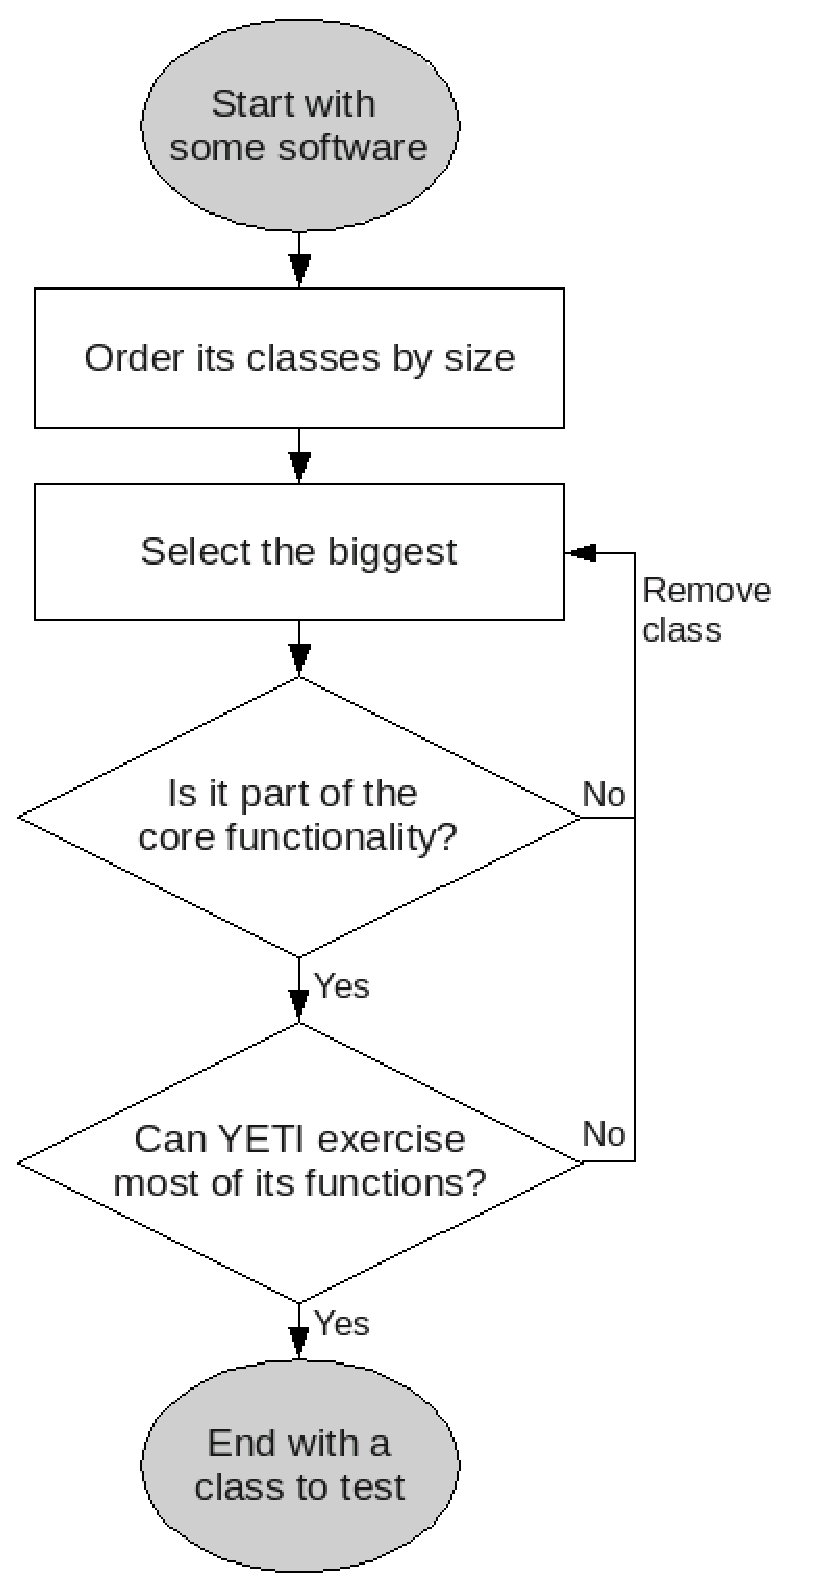
\includegraphics[width=57mm]{figures/flowchart.eps}
\caption{Method to select which class to test}
\label{flowchart}
\end{figure}

This research considers five categories of software application. \emph{Functional} systems involve significant numerical calculation and/or algorithmic operations. \emph{Open} systems have features that are shared between multiple parties, with potentially different goals. \emph{Progressive} systems are used to maintain and develop a data source over time. \emph{User} systems may be command-line, graphical or even web-based. \emph{Timed} systems include a real-time performance requirement and typically some form of concurrency.

\section{Experiments}
Hundreds of thousands of random test cases were applied for every class to provide a basic analysis of the fault characteristics of each application. YETI was used to test each class for ten minutes and record any relevant failures along with the time they occurred. As this required a considerable amount of memory, it was necessary to extend YETI's working memory allowance up to 500 Megabytes. A relevant failure is a failure that has not been seen before. Although the software may fail many times, we are more interested in the relevant failures because they give a better indication of the software's fault characteristics.


\subsection*{Functional}
Functional systems range from core data stuctures such as \emph{java.Integer}, up to complex libraries such as the \emph{Bouncy Castle} cryptography suite. We considered \emph{JBullet}, a full 3D physics environment for Java. JBullet has to process numbers quickly and efficiently, whilst at the same time provide accurate calculations. Figure \ref{functional} shows only two relevant failures were raised by the class, both very early on in the evaluation. This suggests the biggest danger with this type of software is not the occurrence of run-time errors, but rather incorrect calculations or delays that affect the worst case execution time for particular inputs.
\begin{figure}[!h]
\centering
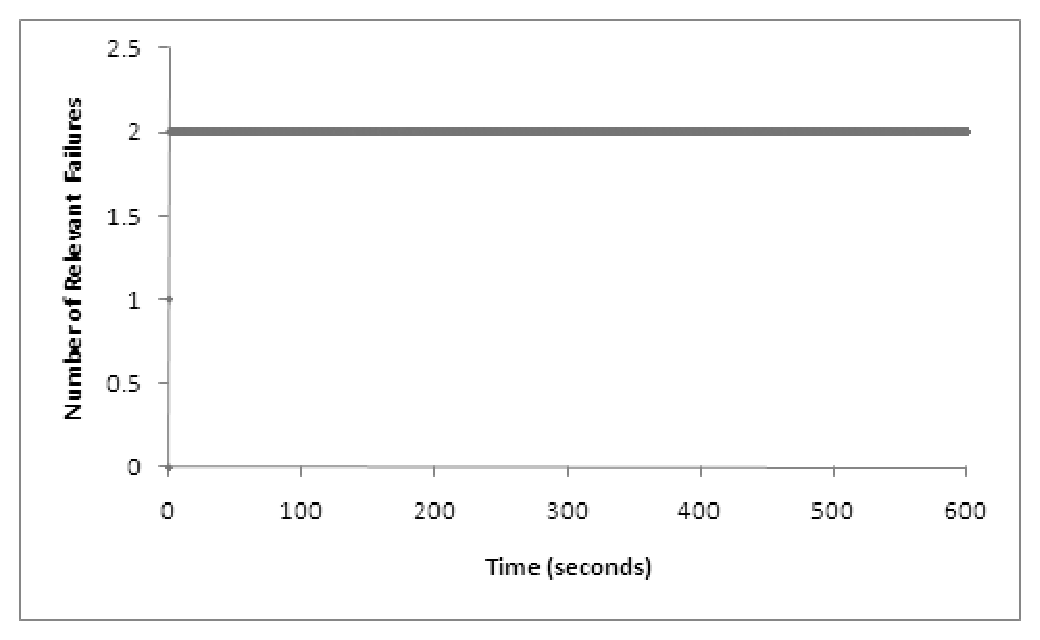
\includegraphics[width=80mm]{figures/functional.eps}
\caption{Functional System Faults}
\label{functional}
\end{figure}


\subsection*{Open}
Open systems face dangers from attackers outside the system and the possibility of conflict between different modules inside the system. It is important that the software possesses fault tolerance and is able to resist tampering. Therefore, it is a surprise to see 19 run-time errors when analysing the \emph{jigsaw.ssi.SSIFrame} class of the Jigsaw web server (see figure \ref{open}). These errors might be masked with the interaction between classes, but they may still cause problems if left unseen. Open systems are particularly prone to problems when there is a heterogeneity of languages, platforms and architectures. This makes it impractical to show software is free from errors. Therefore, it is difficult to make accurate predictions as to the reliability of an open system. 
\begin{figure}[!h]
\centering
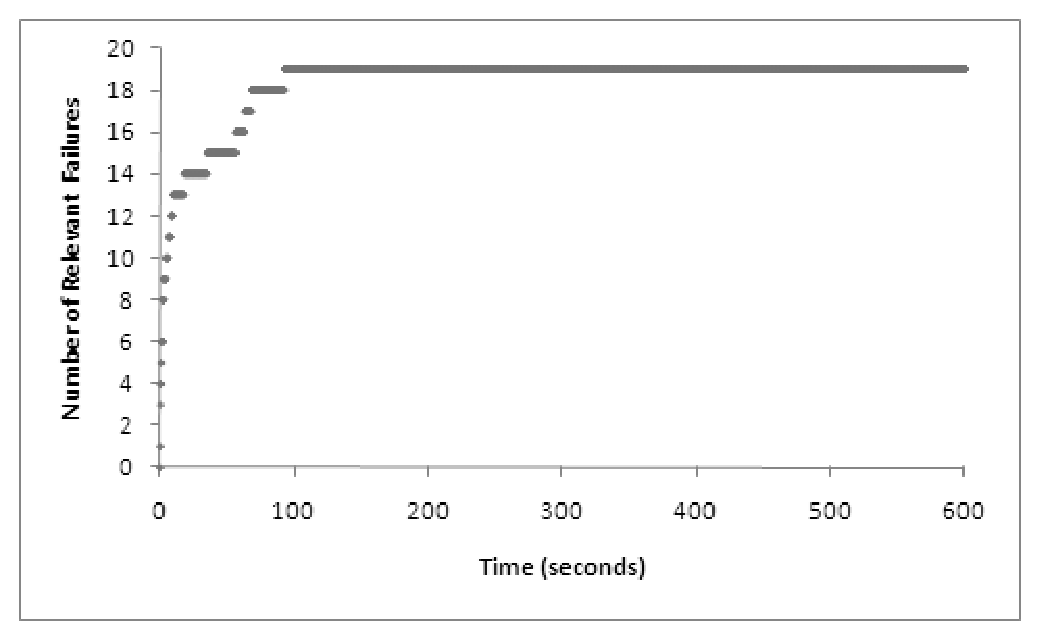
\includegraphics[width=80mm]{figures/open.eps}
\caption{Open System Faults}
\label{open}
\end{figure}


\subsection*{Progressive}
When a progressive system starts with a data source in a particular state, it must leave it in a legal state. This can be difficult, as the data source may potentially be infinite, or only bounded by the available memory. Typically, this is addressed by dividing the data source into manageable sections, for example a byte stream. We investigated the \emph{Apache Derby} database manager and chose the class \emph{org.apache.derby.impl.sql.SQLParser} to investigate. Figure \ref{progressive} shows that 47 relevant failures were found in two stages. The first 40 errors were found very quickly, but it took a while longer before the remaining seven could be found. This suggests that when testing progressive systems, it is important not just to consider a few isolated examples, but to make a thorough investigation using complete case models.
\begin{figure}[!h]
\centering
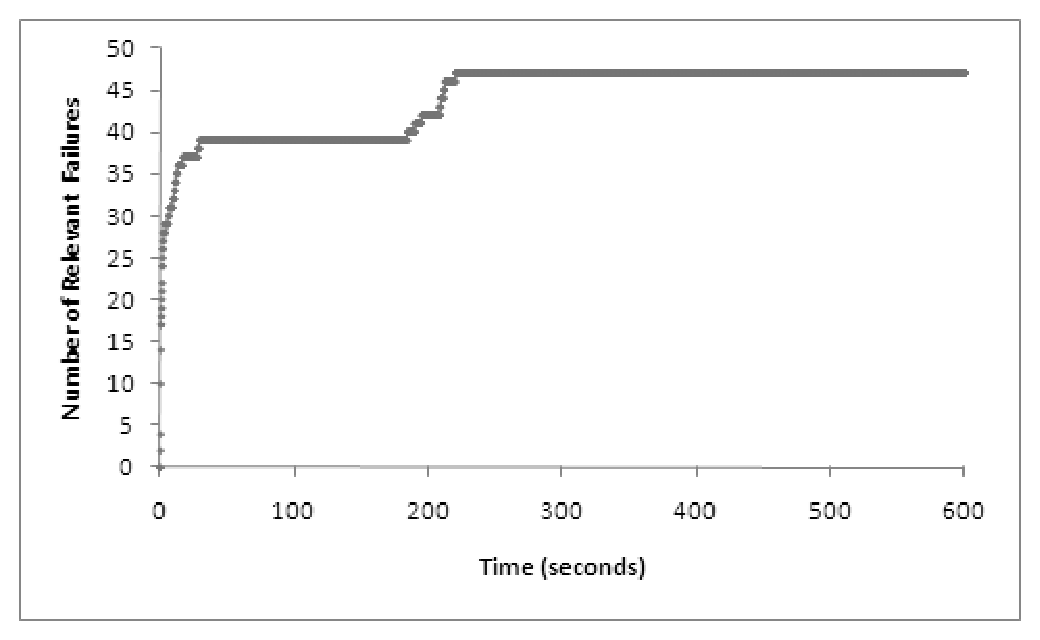
\includegraphics[width=80mm]{figures/progressive.eps}
\caption{Progressive System Faults}
\label{progressive}
\end{figure}

\subsection*{User}
Out of all our experiments, the \emph{javax.swing.JTree} class from Swing generated the most run-time errors. Run-time errors may occur in user systems when an unsolicited GUI event occurs. It is difficult to test the many paths through a user system because of the many ways that interface components can be manipulated. This may be the reason for the steady increase in the number of failures throughout evaluation (see figure \ref{user}). More failures may even have been found if the evaluation was left to run. The biggest challenge in testing this kind of system is being able to cover a sufficient proportion of the search space. This is made even more difficult when we consider there is a human element involved, raising the level of unpredictability.
\begin{figure}[!h]
\centering
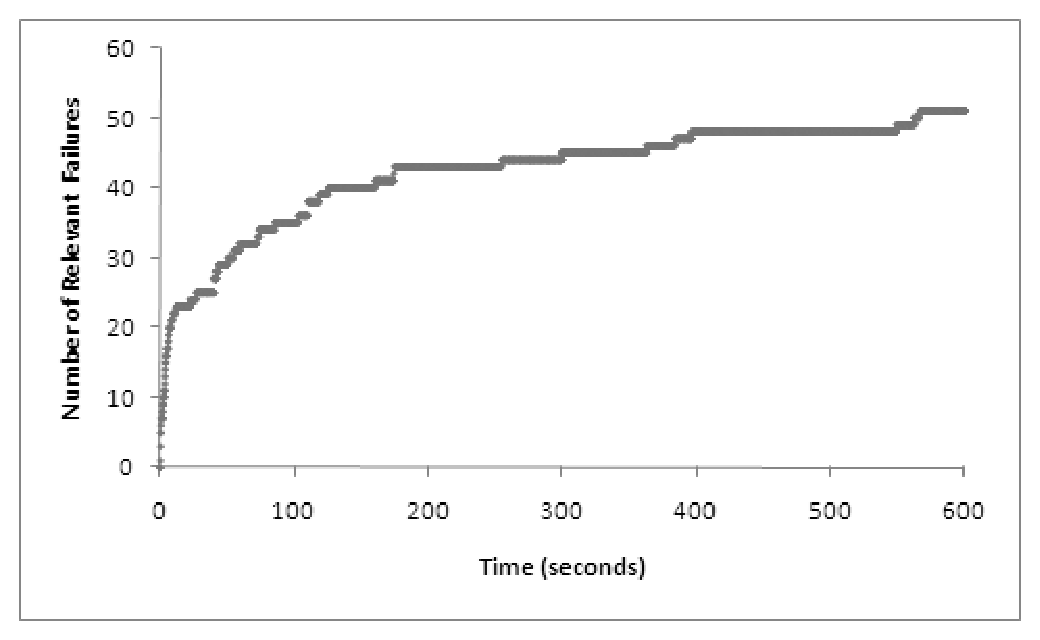
\includegraphics[width=80mm]{figures/user.eps}
\caption{User System Faults}
\label{user}
\end{figure}


\subsection*{Timed}
Finally, we investigated the \emph{javolution.util.FastMap} class of \emph{Javolution}, a real-time library for Java. Failures in timed systems may result in unexpected deadlock and race conditions. These can be difficult to avoid and expensive to detect because they occur as an interaction between classes. Although we were able to find some run-time errors (see figure \ref{timed}, they might not be representative of those that typically occur in timed systems. The errors we found may be common to any library. Therefore, timed systems on the whole can be unpredictable and difficult to test.

\begin{figure}[!h]
\centering
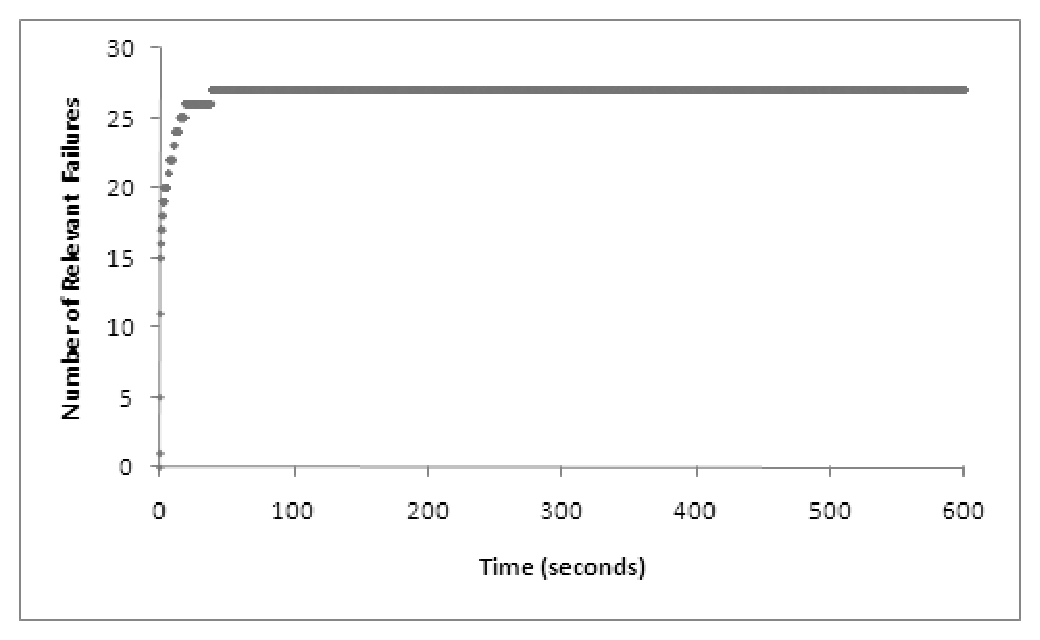
\includegraphics[width=80mm]{figures/timed.eps}
\caption{Timed System Faults}
\label{timed}
\end{figure}



\section{Limitations and Future Work}
We have already mentioned the difficulties involved in finding classes to represent the software under analysis. Some classes are overly specialised and others too generalised to be relevant for this purpose. If a class involves considerable interaction with other classes (for example in a timed system), the inter-class dependencies may be too great for the isolated results from one class to be useful on their own. If this technique is to be used in determining relevant fault characteristics for such software, it will be necessary to adapt it to involve the analysis of more than one class. There is already some support for this in YETI. The next step is to design a process by which a subset of classes may be chosen and the way in which they are to interact decided.

As YETI does not use an explicit oracle, it does not have any real insight as to whether software performs the correct operations. This may be a problem for functional systems, which rely heavily on the notion of correctness. If this is a concern, it should be possible to make use of bug repositories to analyse which particular errors have occurred in the past. However, these may be subjective and time-consuming. One of the main reason for using YETI is that it is able to analyse software for which there is no oracle or for which the specification is inaccurate.

\section{Conclusions}
In conclusion, this technique has been able to identify an interesting characteristic about each category of software. At present it appears unsuitable for certain categories (i.e. functional and timed). However, this may be corrected by including more classes in the analysis. Although random testing may struggle to find a particular failure that occurs only for a small subset of the input domain, it can run many test cases quickly and should be able find most of the failures with relatively little computational expense. The biggest challenge for the future will be to determine how to choose which combinations of classes should be exercised together for optimum results. If this can be achieved, random search could be an excellent choice for identifying the failure characteristics of software.


\begin{thebibliography}{5}

\bibitem{ince_1987} Ince, D., The automatic generation of test data. The Computer Journal. 30:1, 63--69 (1987)
 
\bibitem{myers_2004} Myers, G., Badgett, T., Thomas, T. and Sandler, C., The Art of Software Testing, Wiley, New York (2004)

\bibitem{hamlet_1994} Hamlet, R., Maciniak, J., Random Testing, Encyclopedia of Software Engineering,  Wiley, New York, 970--978 (1994)

\bibitem{mankefors_2003} Mankefors, S., Torkar, R. and Boklund, A., New quality estimations in random testing, Proceedings of the 14th International Symposium on Software Reliability Engineering, 468--478 (2003)

\bibitem{microsoft_2010} Microsoft Corporation, Software Categories, Microsoft TechNet, http://technet.microsoft.com/en-us/library/bb852143.aspx (2010)

\bibitem{oriol_2010} Oriol, M., Testing .NET Code with YETI, Proceedings of the 15th IEEE International Conference on Engineering of Complex Computer Systems (2010)

\end{thebibliography}


\end{document}
